\chapter{Implementation}
\label{chap:chapter4}
In this chapter we are going to show a concrete implementation of the architecture explained previously. For each layer we will provide explaination of the most important features using diagrams and code snippets.

\section{AWS Deploy}
elencare le macchine usate e come sono stati deployati i vari servizi su di esse
mettere configurazioni?

\section{Data ingestion}
TV2 runs Sumo production envirovment into a virtual private cloud on Amazon Web Service (AWS), isolated from the outside network and it is not possible to fetch them directly. A typical cloud production envirovment keeps the virtual machines inside private networks and routes the network traffic to the external network through NAT instances. A bastion server is normally placed as protection against undesidered accesses such that only trusted user can access the private cloud. \\

Since Sumo platform uses Apache Kafka as a message sharing system between several services, it has been convenient and easy to create a "data bridge" inside that envirovment for pushing data inside the VimondAnalytics one. \\
For this purpose it has been used an already existing Vimond project called "Firehose", which has been modified for this use case. Firehose simply implements a two endpoints system. Data are read from a Kafka topic, validated and forwarded to another Kafka cluster. For security reason, Firehose is installed on a machine inside TV2 VPC: in this way the Kafka cluster source is directly accessible throught private IPs. In order to connect it to the VimondAnalytics Kafka cluster, an elastic IP is assagned to the latter.

\begin{figure}[h]
        \centering
        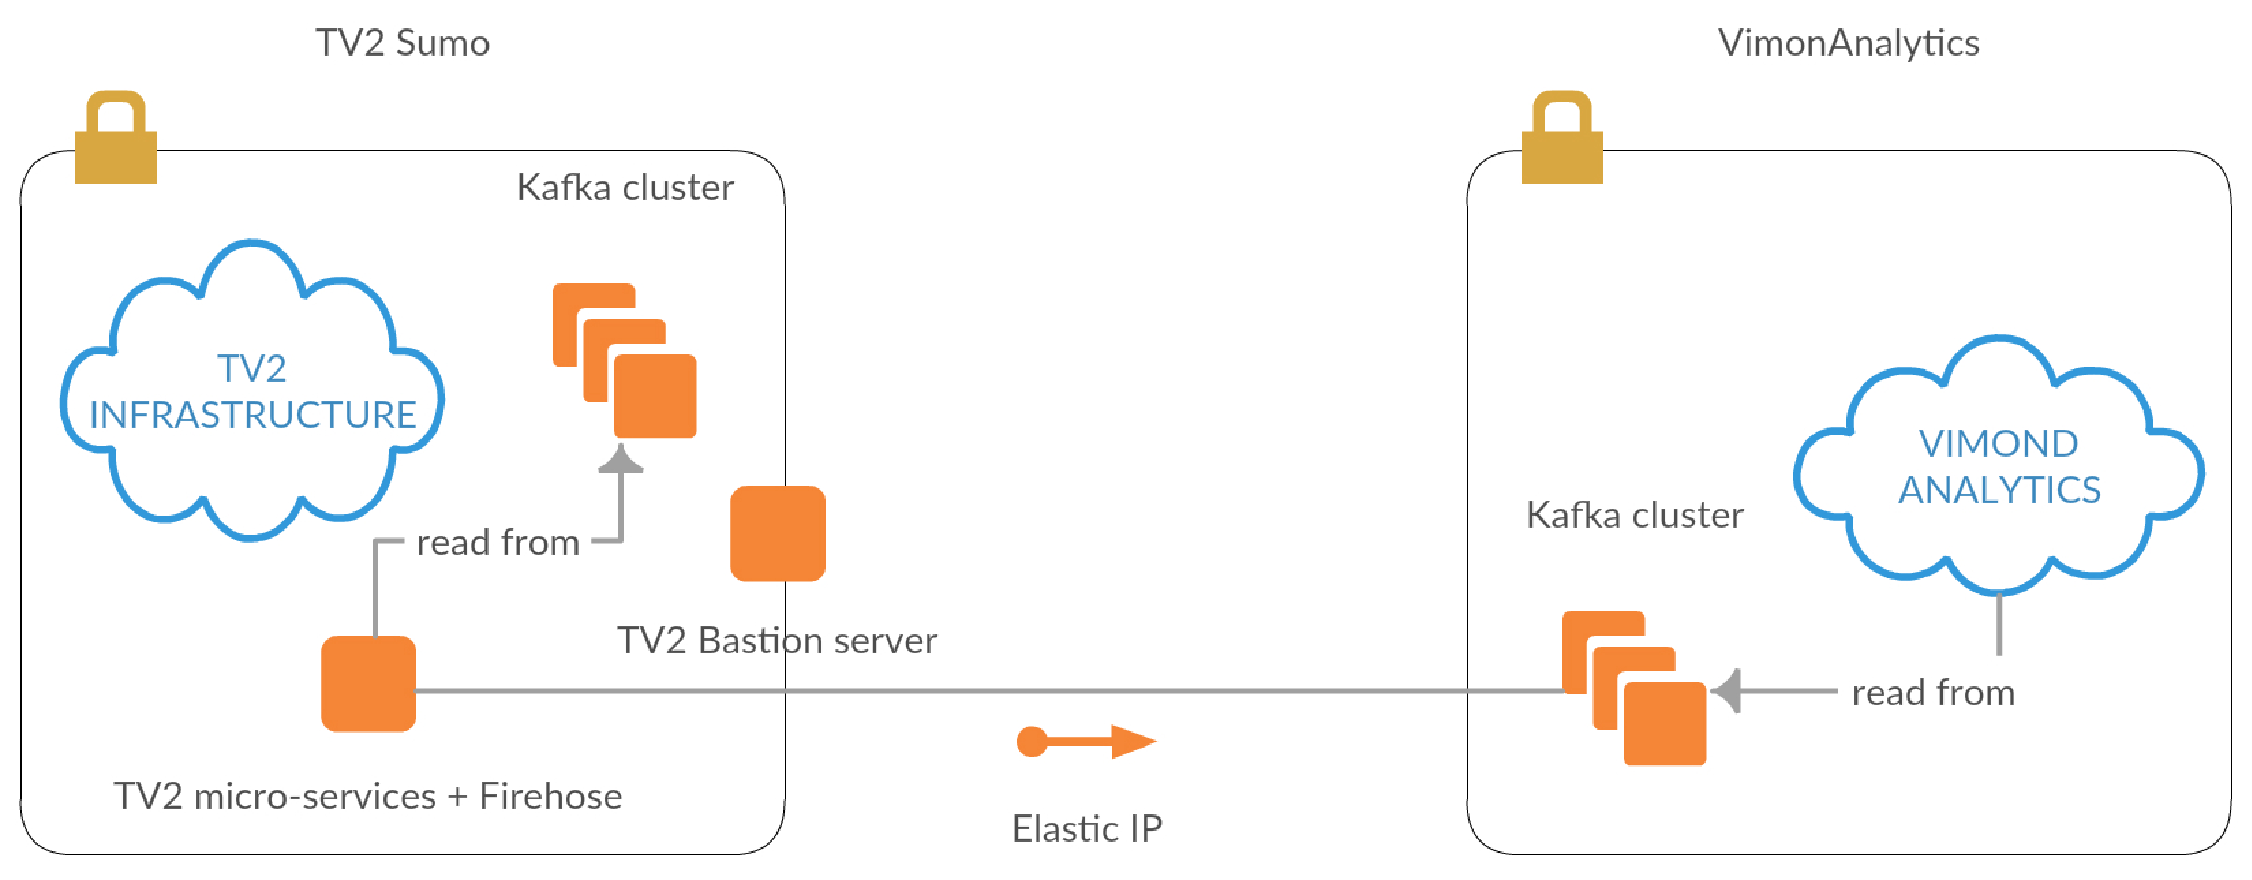
\includegraphics[width=12cm]{imgs/Firehose.pdf}
\caption[Firehose data bridge]{Firehose data bridge}
        \label{firehose-1}
\end{figure}

\subsubsection{Data model}
As said in the previous chapter, the data used for this project come from the resume player functionality provided by TV2 pay-per-view platform \textit{Sumo}. Data are generated by players running on different devices: it results in two type of events according to the usage of silverlight plugin. The events generated by other plugins contains a subset of information of the ones generated by silverlight plugin. Specifically, an example of non-silverlight event is:
\begin{listing}
\begin{minted}[frame=single,
               framesep=3mm,
               linenos=true,
               xleftmargin=21pt,
               tabsize=4]{js}
               
{     
    "eventName":"player_log_event"
    "originator":"player"
    "timestamp":"2015-09-13T10:31:39.879Z"
    "guid":"5d33aa50-8232-447e-8b5a-14b4317f1265"
    "progress":
    {
    	"assetId":958291
    	"title":"God morgen Norge"
    	"offset":
    	{
    		"duration":7133249
    		"pos":7101143
    	}
    	"category":
    	{
    		"id":919990
    		"name":"Innev?rende sesong"
    	}
    }
}               
\end{minted}
\caption{Non silverlight event example} 
\label{nosilveright-example}
\end{listing}

\newpage
In addition to these information, an event generated by silverligth plugin contains an additional field with details about the client used for playing a particular asset. In listing \ref{silveright-example} we reported the most important fields for our analysis.

\begin{listing}
\begin{minted}[frame=single,
               framesep=3mm,
               linenos=true,
               xleftmargin=21pt,
               tabsize=4]{js}
               
{     
    "client":
    {
    	"playerEvent":"period"
    	"userAgent":"Mozilla/5.0 (Windows NT 6.1; WOW64; rv:40.0) 
    	Gecko/20100101 Firefox/40.0"
    	"env.platform":"silverlight"
    	"buildName":"Vimond.Player.TV2Sumo"
    	"video.format":"smil"
    }
}               
\end{minted}
\caption{Silverlight event example} 
\label{silveright-example}
\end{listing}


\section{Output results}
One of the limit of lambda architecture is that the output needs to be defined a priori. Accorting to the considerations made in section \ref{chap3:consideration}, the following output views has been defined:
\begin{enumerate}
\item Number of times of assets starting or ending. 
\item Most started assets.
\item Most ended assets.
\item Most browsers used when starting an asset.
\item Most OSs used when starting an asset.
\item Most video formats used when starting an asset.
\end{enumerate}
In order to have consistent outputs across the different batch views we exploit the field \textit{"playerEvents"} which gives information of the type of event performed by the user. It can assume the values \textit{start}, \textit{period} and \textit{end}. We could not use the event marked with \textit{period} as the different batch windows does not share information and then every results produced out of them would have not been consistent. A \textit{playerEvent=start} or \textit{playerEvent=end} represents instread a unique event. Unfortunately, only a subset of the imput data contains information about the player event (i.e. the one generated by the silverlight plugin). A request has been forwared to TV2 for having these information also in the events generated by other devices. Moreover it has been requested to change the mode of generating \textit{end} events: an user likely stops the streaming of an asset before it actually ends, for instance when skipping the ending titles, and this results in a smaller number of this kind of events. An alternateve solution would be to consider an asset to be ended when the streaming reached a certain percentage over its lenght, for instance 95\%. These features are going to be implemented within the next platform release.

\section{Batch layer}

\subsection{EventFetcher}
EventFetcher is the process in charge of reading events from Kafka a store them in the HDFS according to their timestamp. There are two different execution mode: unreliable and realiable. Figure \ref{EF-Class} shows the class diagram for the main classes involved, reporting the most important fields and methods.
\begin{figure}[h]
        \centering
        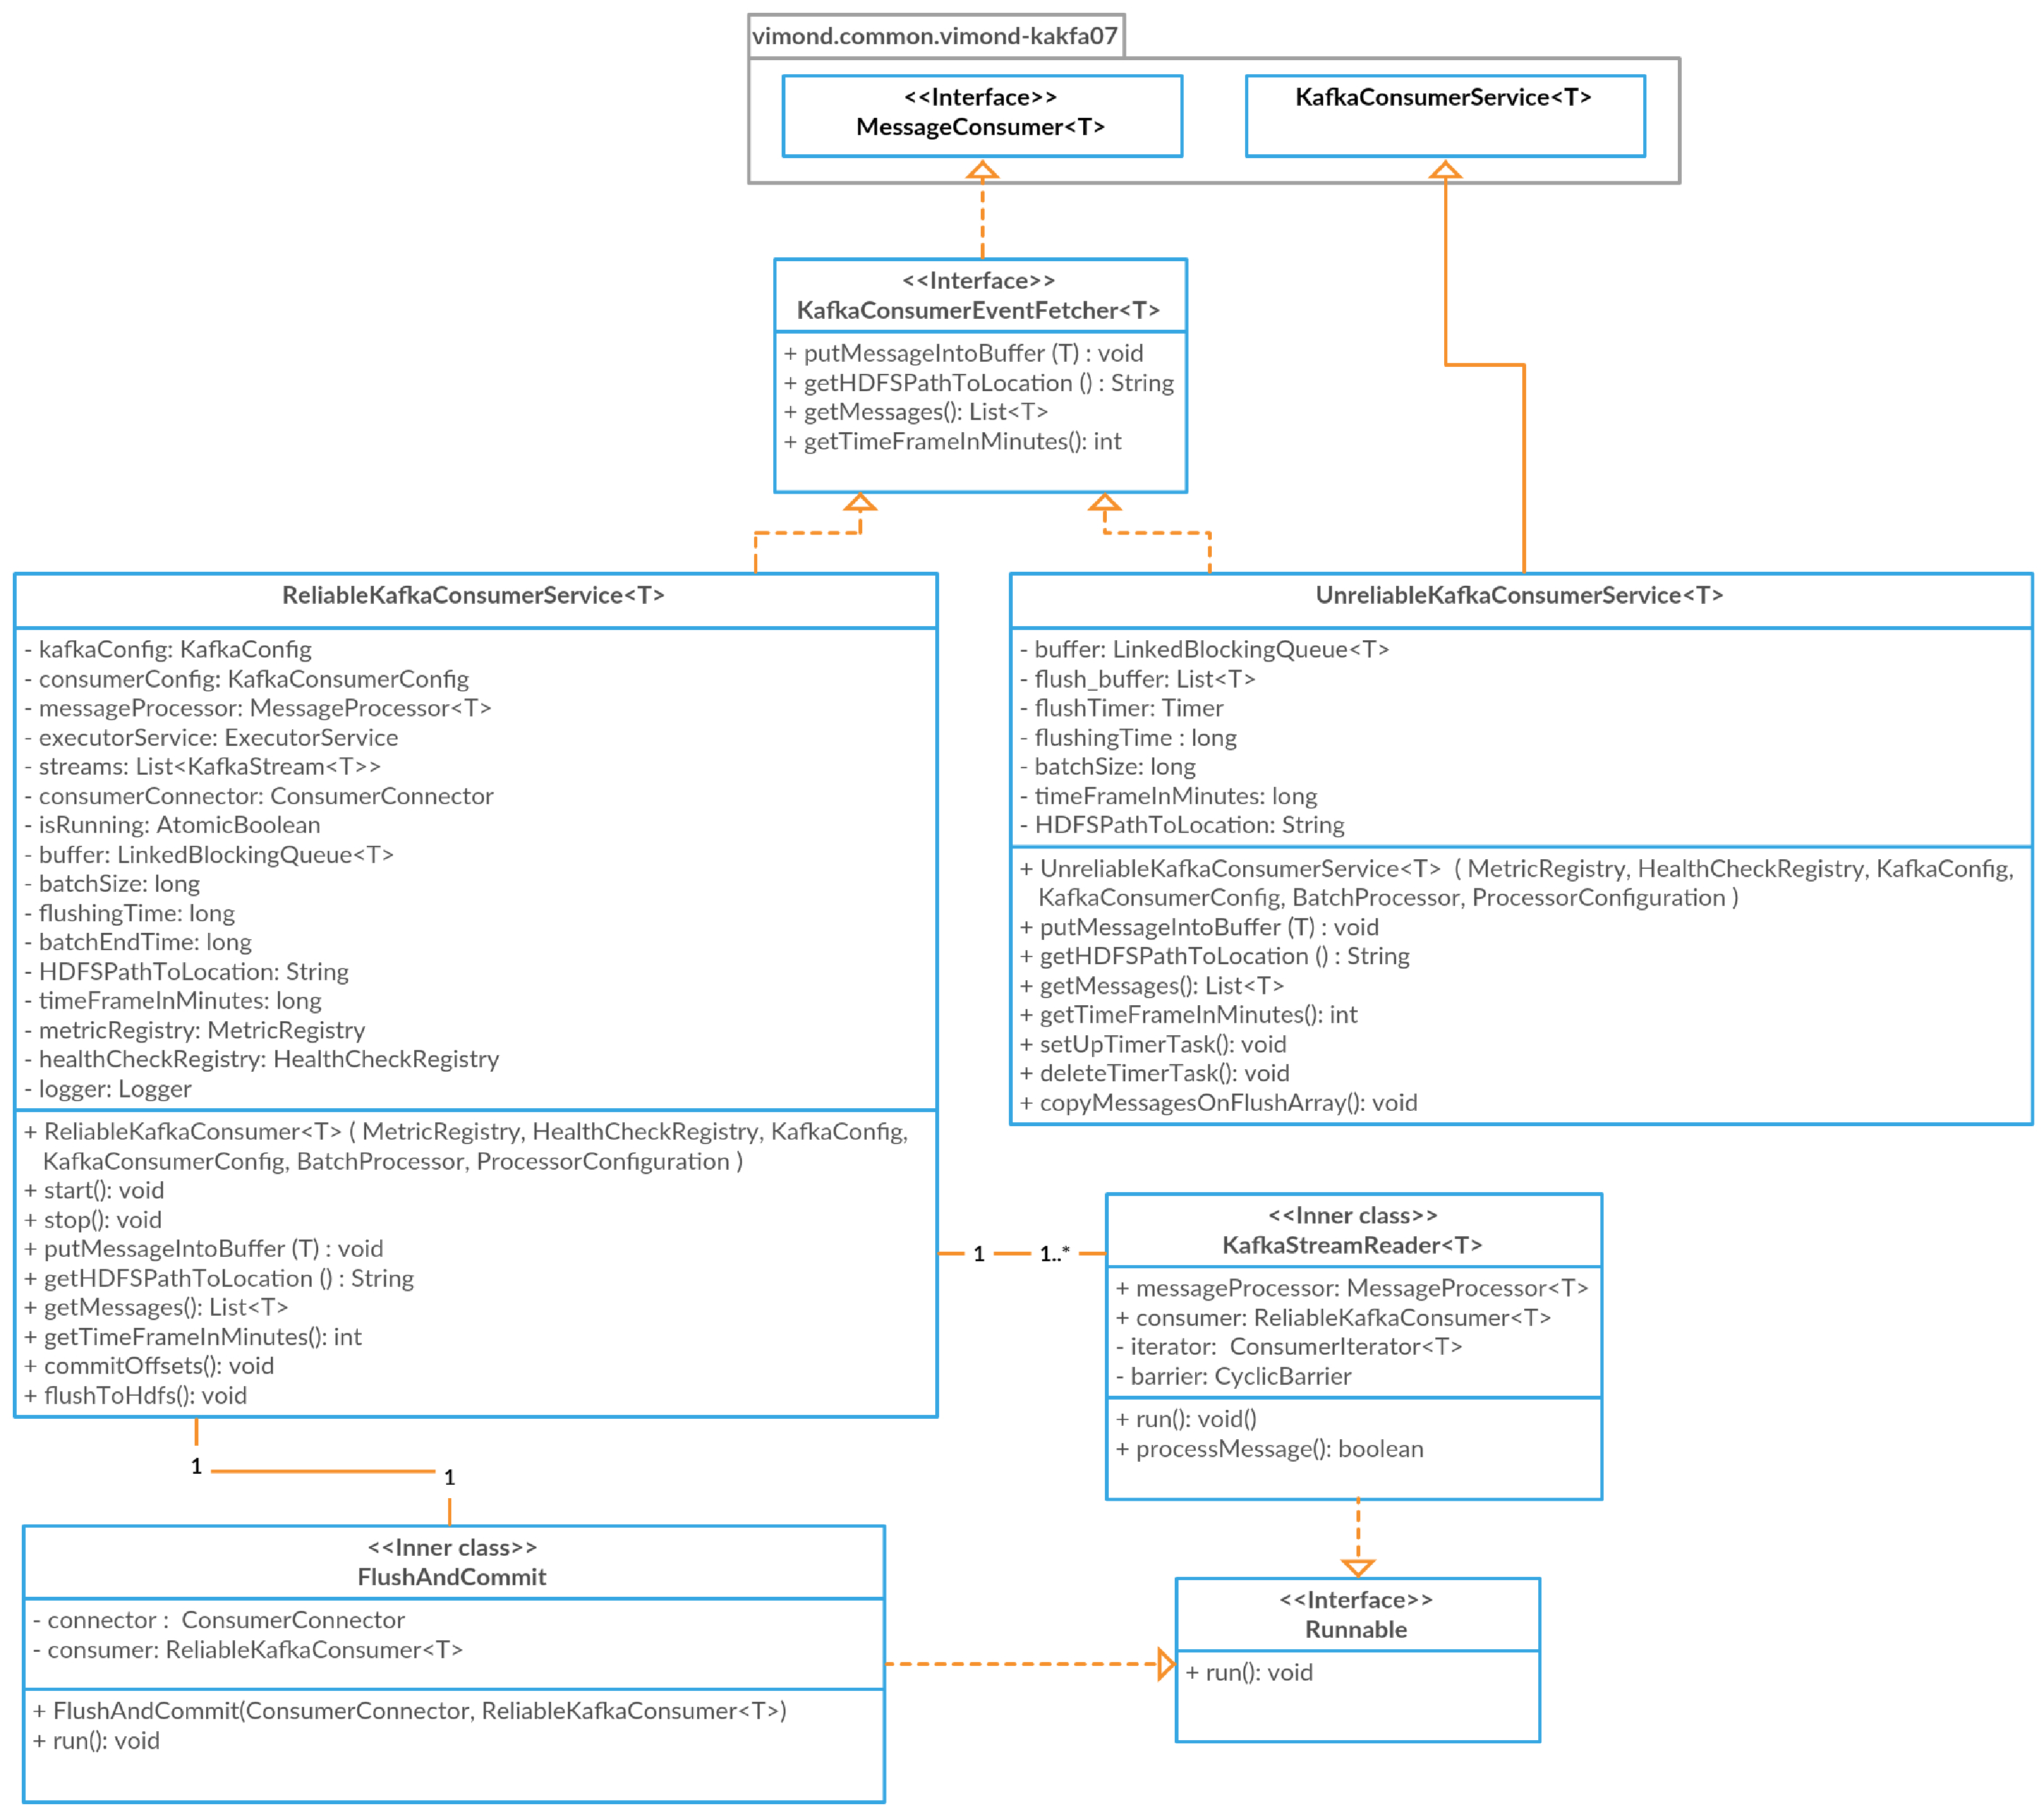
\includegraphics[width=15cm]{imgs/eventfetcher-uml}
\caption[EventFetcher class diagram]{EventFetcher class diagram}
        \label{EF-Class}
\end{figure}

The \textit{UnreliableKafkaConsumerService} extends a kafka consumer class defined in the Vimond repository since the latter offers method for reading messages from a kafka brokers and committing the offset immediately after. What was missing was the ability to process the messages in batches. Each consumer threads reads from kafka and puts the message in a \textit{LinkedBlockingQueue}. The usage of this object is due to its thread-saftness. Each batch operation is triggered either by time or by a threshold on the number of messages stored in memory. Whenever one of this events occurs, the messages are copied into a separate buffer and written in batch into the HDFS from a separate task. This ensure that the storing messagest is not a bottleneck in the overall process, but does not give any guarantees about the correct execution of the operation since the consumer threads are not aware of the writing one.\\
The \textit{ReliableKafkaConsumerService} instread, behaves similarly to the unreliable counterpart, but does not commit a message offset after reading it, only when a batch has been successfully written on HDFS. All the consumer thread are synchronized by a \textit{CyclicBarrier} object. Every time a message is reveived, it is stored in a common buffer and each consumer thread checks if the message threshold or a batch interval has been reached and in case blocks itself on the barrier. The last thread to complete these operations is the one delegated to write the messages into the HDFS: it first tries to contact the HDFS namenode and, in case of its availability, it proceeds with the writing part. In case the namenode is not available, for instance due to a network error, it keeps retrying to contact it using an exponential backoff policy. When the writing process is completed, the offset is finally committed since that batch of messages is considered processed. In order to avoid deadlock, the other threads waits on the barrier for no more than a configurable time, after that, the overall programs raise an exception and exits. This is not the best approch even though guarantees that the next execution of the program reads the same messages that otherwise could have been lost. 

\subsection{Batch data pipeline}
As we said before, we used Apache Spark for implementing this layer. Spark itself does not provide any scheduling mechanism but just a single execution of the aggregation process. Normally an action scheduler is needed for the repetition of the same batch job, each time parametrized in a different way. Considering the usage of Hadoop HDFS as a solution for the data storage, it resulted convenient using Apache Oozie, the official job scheduler over Hadoop. As we explained in chapter \ref{chap:chapter2}, Oozie allows to schedule a DAG of actions, where an action is executed only when the previous one ended.\\
\begin{figure}[h]
        \centering
        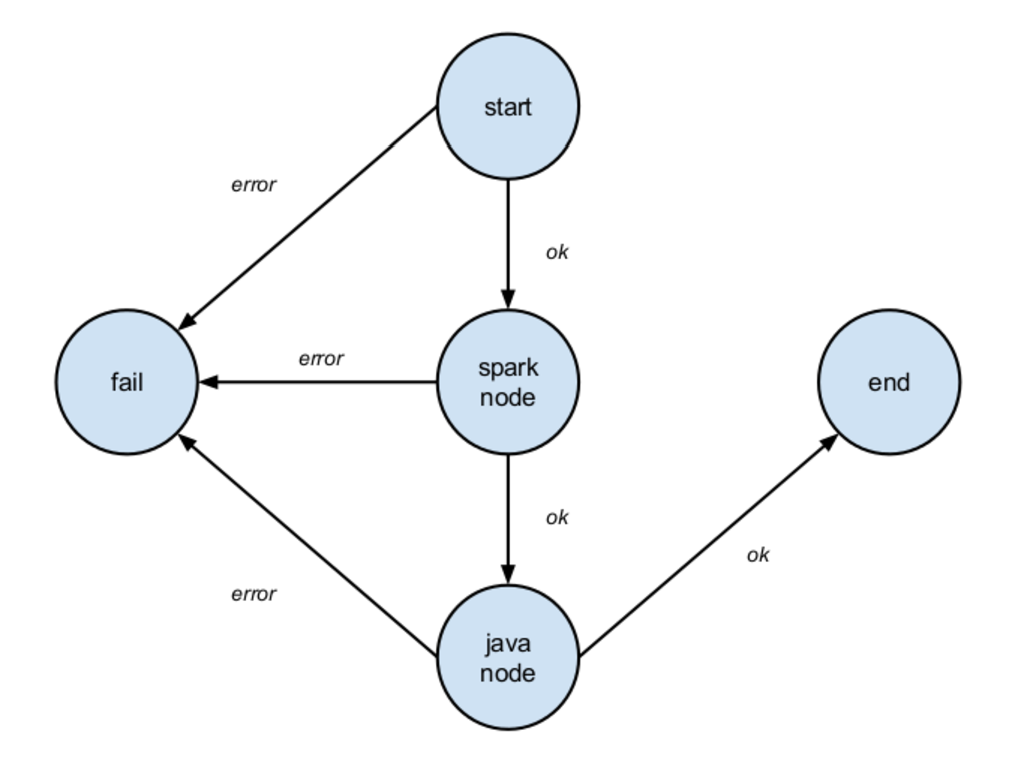
\includegraphics[width=12cm]{imgs/Oozie-DAG.pdf}
\caption[Oozie data pipeline]{Oozie data pipeline}
        \label{oozieDAG}
\end{figure}
Picture \ref{oozieDAG} shows the sequence of actions performed at every execution:
\begin{itemize}
\item start, fail and end are control nodes.
\item spark-node and java-node are action nodes.
\end{itemize}
The user specifies the input parameters such as the beginning time or the frequency of the execution through a property file containing a list of \textit{key=value} tuple.
A execution of the DAG is defined through an XML file called \textit{workflow.xml}, while the scheduling is defined though  a \textit{coordinator.xml} file. Oozie allows to define parametrized paramenter which are resolved with a different value according to the current execution: in this case the job takes a different input folder according to the time of the execution as showed in listing \ref{oozie-example}.
\begin{listing}
\begin{minted}{xml}
<datasets>
	<dataset name="vimondEvents" frequency="${coord:minutes(30)}" 
	initial-instance="${datasetStartTime}" timezone="GMT+02:00">
	<uri-template>${nameNode}/user/${coord:user()}/${datasetFolder}
	/master/${YEAR}-${MONTH}-${DAY}/${HOUR}/${MINUTE}</uri-template>
	</dataset>
</datasets>
<input-events>
 	<data-in name="input" dataset="vimondEvents">
  		<instance>${coord:current(-2)} </instance>
	</data-in>
</input-events>
\end{minted}
\caption{RealTime data example} 
\label{oozie-example}
\end{listing}

With the \textit{dataset} tag it is possible to define a parametric path where to take the data according to the \textit{YEAR-MONTH-DAY/HOUR/MINUTE} pattern. A dataset can an input or output one. In this case, with the tag \textit{data-in} we consider an input dataset resolved into the dataset generated two batch window before the current execution. For instance, let assume to have a 30 minutes batch window and let the next to be executed at 17 pm of a certain day: that job will work on the dataset containing the data from 16:00 to 16:30. This is a complication derived from kafka: since it does not ensure message ordering we cannot be sure that at the time of the execution of a job, all the events of the previous timeframe has been written on the correct folder. We have checked empirically that, delaying the execution of a job of two timewindows guarantees that all the events are considered in the execution.\\
After the validation of the input parameters, the execution continues throught the spark node. This is the step where raw data are actually analyzed and aggregated in order to have a compact view on them. Since we already use Hadoop, in oder to avoid the deployment of another processing system, we decided to run Spark jobs on Yarn. As stated in chapter \ref{chap:chapter2}, Yarn is indipendent from the computing paradigm as it only allocates resources to containers which make requests for them. There are two modalities of running Spark on Yarn: \textit{client-mode} and \textit{cluster-mode}. In the first one, the Spark driver program is run on the client while in the last one the driver runs within the same container of the Application master. \\
The program written using Spark library does a strong use of in-memory capability of the framework. The following picture represents the steps executed within the program.
\begin{figure}[h]
        \centering
        \includegraphics[width=12cm]{imgs/spark_DAG.pdf}
\caption[Spark actions]{Spark actions}
        \label{sparkDAG}
\end{figure}

Spark provides for methods for loading binary data directly from HDFS, so no effort is required for converting byte arrays in String. Every loaded event is then converted into a \textit{SparkEvent} object for being analyzed. 
Since Kafka offers an \textit{at-least-one} message semantic, there might be duplicates, hence an additional filter process is then needed in order to remove them. Unfortunately this is the most expensive step as it has to analyze the whole dataset, and normally shuffle operations between the executors are needed. The dataset obtained in this step (LOAD DATA block) is then cached in memory since it is needed by every other process yet to be run in the current execution. In case of dataset bigger than the memory available, it is spilled to the disk and deleted when it is no longer needed.\\
From this dataset, three branches are executed:
\begin{itemize}
\item Counter events type: this step calculates the number of start and end events 
\item End events per asset: this step calculates how the end events are distributed among the assets, i.e. what are the assets that users watch till the end
\item Start events: this step is just an additional filter over the loaded dataset. Only player start evets are considered. From the output of this process are executed four additional steps which calculate what are the most used browsers, operative systems, video formats and assets.
\end{itemize} 
All the branches eventually write data on the serving layer in form of JSON events.\\
The aggregation processes are quite simple as they are composed only of map and reduce operation over the dataset. For completion we report a pseudocode of the process who calculates the number of player-end event per asset. \\
\begin{algorithm}[H]
\KwIn{AllEvents input}
\KwResult{Aggregated data written on the serving layer}
\DontPrintSemicolon
\Begin{
$endEvents \leftarrow emptyRDD()$\\
\ForEach{event $e$ in input }{
\If{$e.playerEventType == end$}
			{
				$endEvents.add(e)$\
			}
}
$pairEvents \leftarrow emptyRDD()$\\
\ForEach{event $e$ in endEvents }{
$tuple \leftarrow (event.assetName, 1)$\\
$pairEvents.add(tuple)$
}
$reducedEvents \leftarrow emptyRDD()$\\
\ForEach{tuple $x, y$ in pairEvents }{
\If{$x.assetName == y.assetName$}
			{
				$reducedTuple \leftarrow (x.assetName, x.counter + y.counter)$
				$reducedEvents.add(reducedTuple)$
			}
}
$outputData \leftarrow emptyRDD()$\\
\ForEach{tuple $x$ in reducedEvents }{
$output \leftarrow createBatchData(x)$
}
$writeDataOnServingLayer(outputData)$
}
\caption{End events per assset aggregation\label{IR}}
\end{algorithm}
\bigskip
This is just an example of how output data are generated, the process itself does not iterate several times on all the datasets but exploits the distributed power provided by Spark. A dataset is divided in several partition and distributed on all the working processes which execute the pseudocode above illustrated on a smaller sub dataset, fetching data from other partitions only when needed. 

\begin{figure}[h]
        \centering
        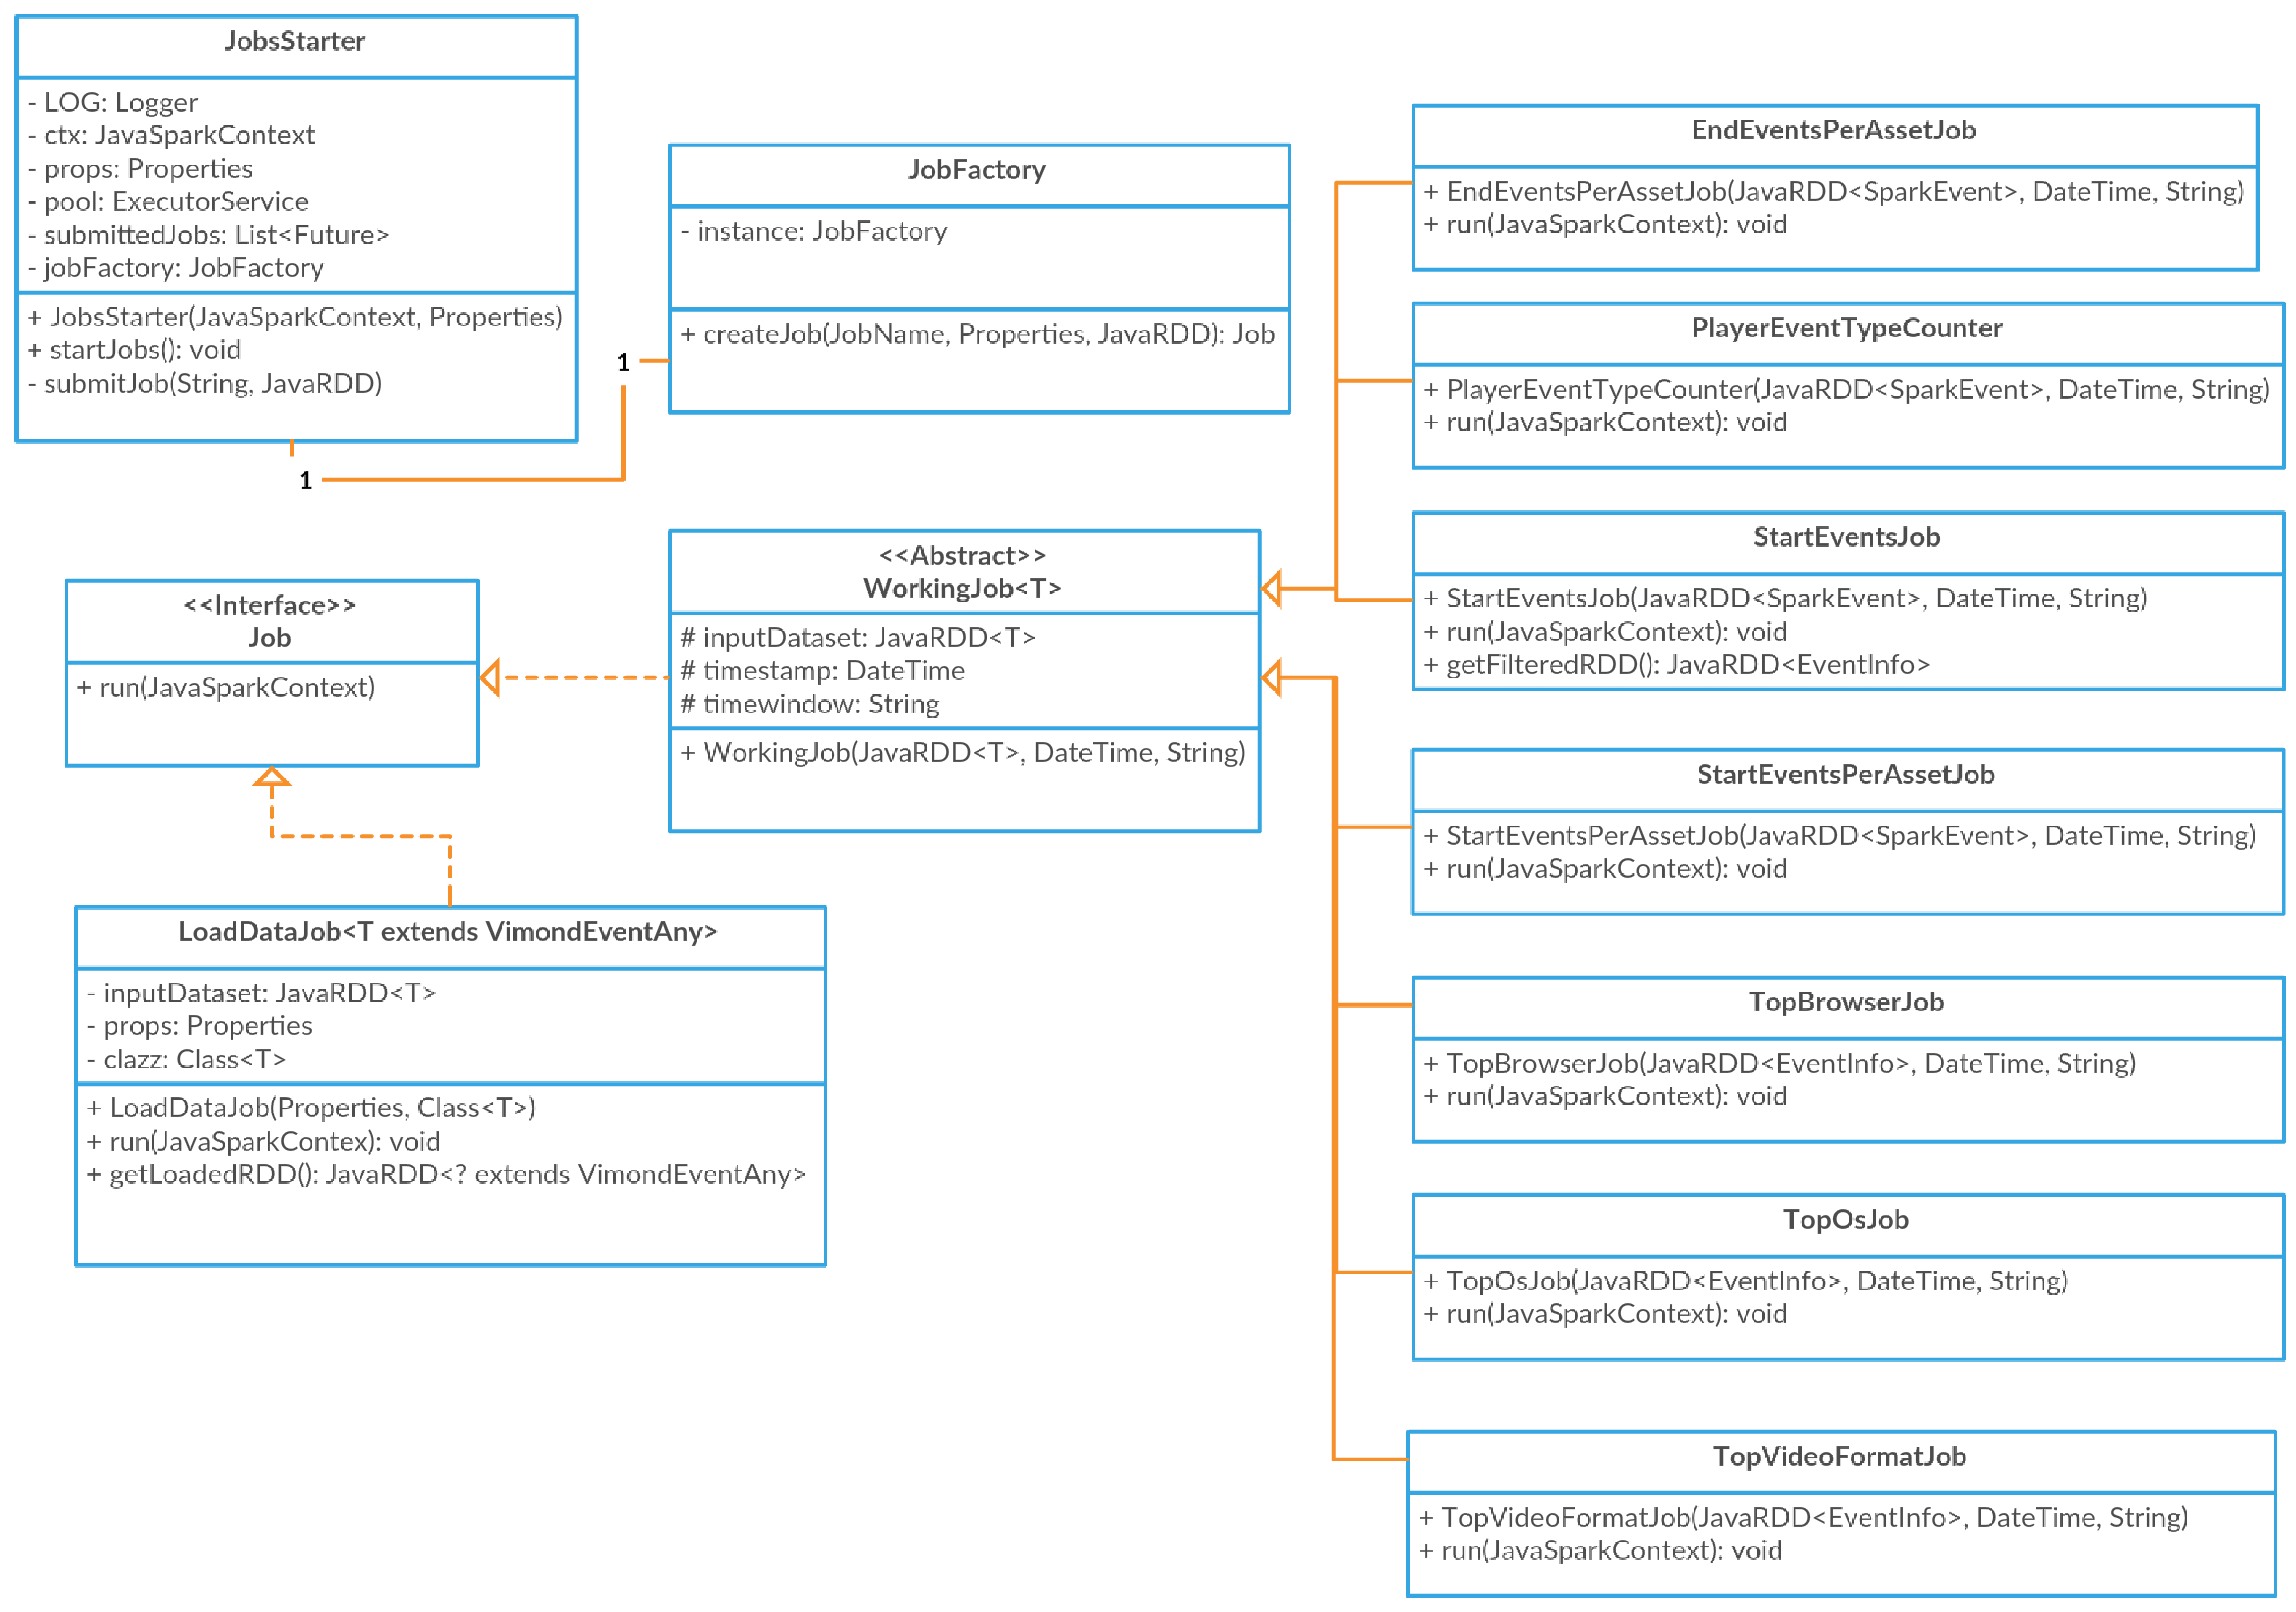
\includegraphics[width=15cm]{imgs/spark-uml.pdf}
\caption[Batch class diagram]{Batch class diagram}
        \label{sparkUML}
\end{figure}

Figure \ref{sparkUML} shows a class diagramm for the most important classes involved in the aggregation process. An aggregation action has been mapped into a Java object implementing the \textit{Job} interface. In addition, for the processes using an input dataset, it has been defined an abstract class named \textit{WorkingJob}. Finally, jobs are started through a \textit{JobStarter} object which uses a factory pattern for jobs creation.

The last step of the batch pipeline is the deletion of the realtime data after the completion of a batch aggregation process over a timewindow of data. This is simply obtained by quering the the serving layer for the data contained in the current time interval and then delete the corresponding results. The serving layer implemented with elasticsearch does not support SQL-like delete operations as \textit{DELETE from table WHERE condition}, but it requires the \textit{id} of the document to be deleted. This process is done in batches in order to improve the throughput of the operations as it would be network expensive sending a delete request for each document. The overall process goes under the name of \textit{delete-by-query}.

\section{Real time layer}

\begin{figure}[h]
       \makebox[\textwidth][c]
       {
        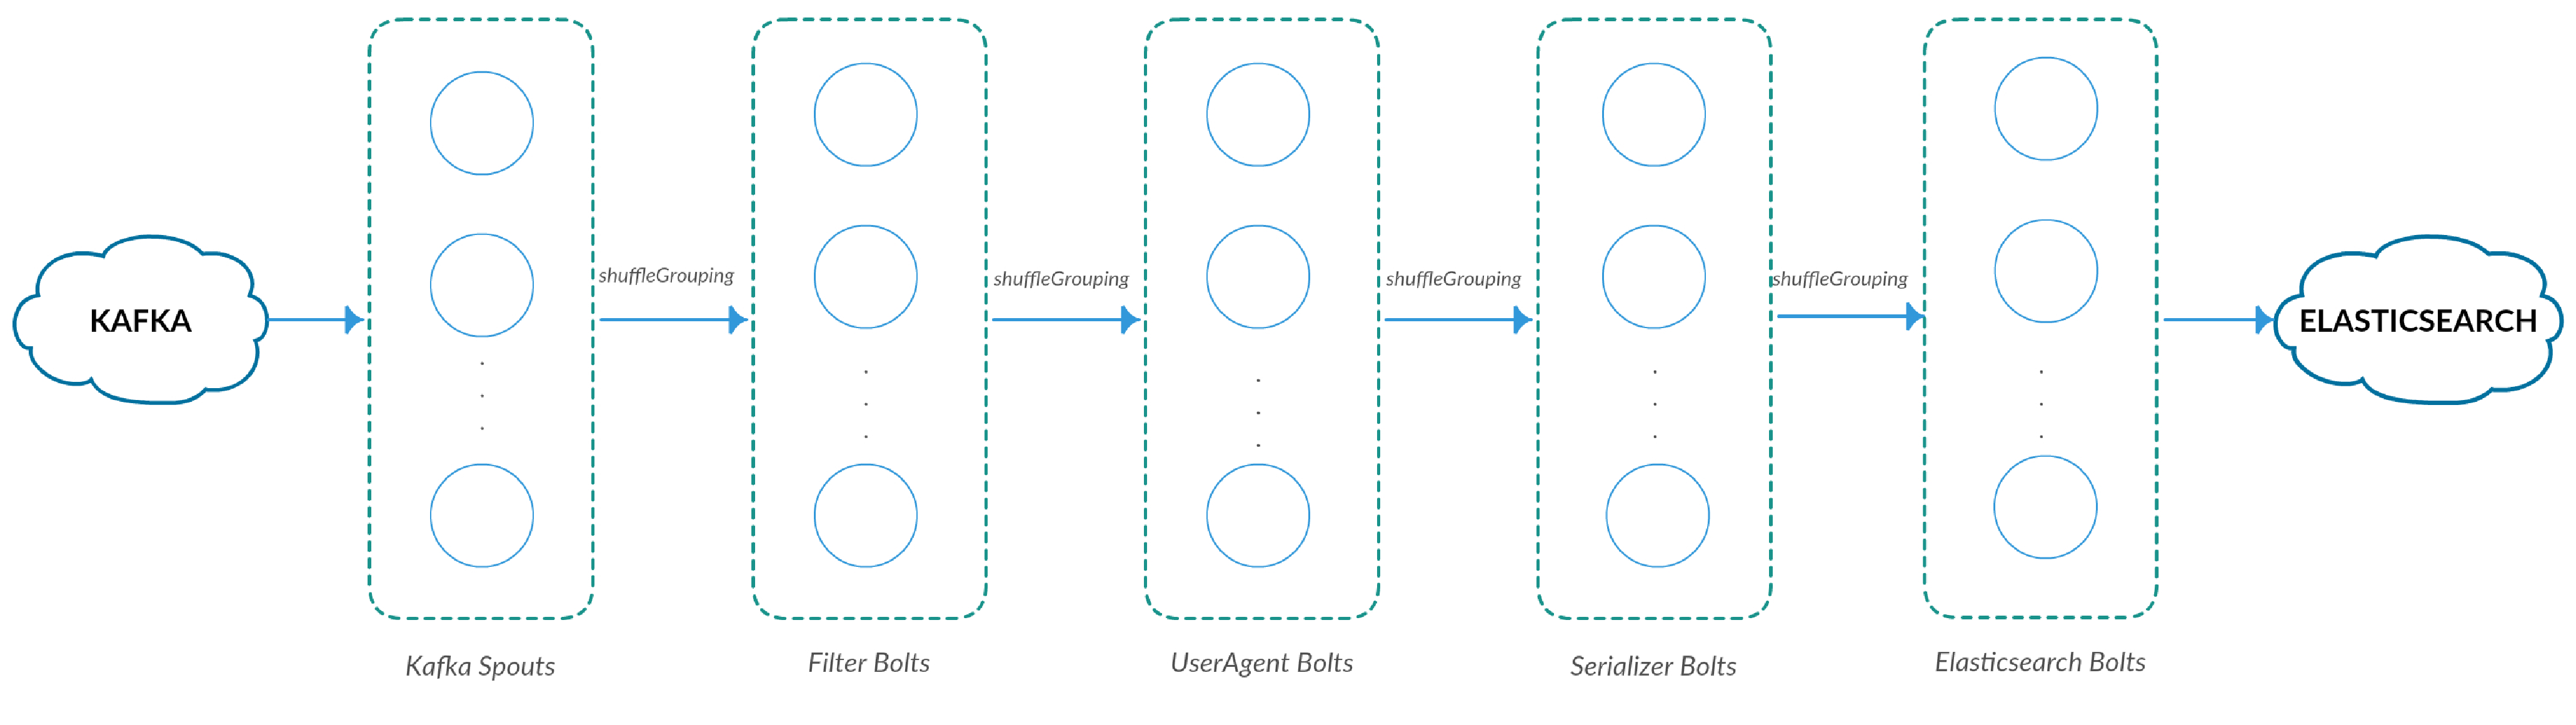
\includegraphics[width=17cm]{imgs/stormTopology}
        }
\caption[Storm real-time topology]{Storm real-time topology}
        \label{stormTopology}
\end{figure}

\section{Serving layer}
The serving layer has been implented using Elasticsearch. As stated in chapter \ref{chap:chapter2}, Elasticsearch provides storage space for documents and a \textit{Lucene} search engine for querying them. Moreover it works with documents in JSON format, making easy to query and aggretate them according to a specific field inside them.

Mapping.\\Query\\Kibana

\section{Tuning}
\subsection{RealTime}
Serialization with kryo rather than objectmapper. show benchmark analysis  on serialization libraries

